% ----------------------------------------------------
% DAB Standard
% ----------------------------------------------------
\documentclass[class=report,11pt,crop=false]{standalone}
% Page geometry
\usepackage[a4paper,margin=25mm,top=25mm,bottom=25mm]{geometry}

% Font choice
\usepackage{lmodern}

% Use IEEE bibliography style
\bibliographystyle{IEEEtran}

% Line spacing
\usepackage{setspace}
\setstretch{1.20}

% Ensure UTF8 encoding
\usepackage[utf8]{inputenc}

% Language standard (not too important)
\usepackage[english]{babel}

% Skip a line in between paragraphs
\usepackage{parskip}

% For the creation of dummy text
\usepackage{blindtext}

% Math
\usepackage{amsmath}

% Header & Footer stuff
\usepackage{fancyhdr}
\pagestyle{fancy}
\fancyhead{}
\fancyhead[R]{\nouppercase{\rightmark}}
\fancyfoot{}
\fancyfoot[C]{\thepage}
\renewcommand{\headrulewidth}{0.0pt}
\renewcommand{\footrulewidth}{0.0pt}
\setlength{\headheight}{13.6pt}

% Page geometry
\usepackage[a4paper,top=25mm,bottom=25mm]{geometry}

% Epigraphs
\usepackage{epigraph}
\setlength\epigraphrule{0pt}

% Hyperlinks & References
\usepackage{hyperref}
\hypersetup{
    colorlinks=true,
    linkcolor=blue,
    filecolor=blue,      
    urlcolor=blue,
    citecolor=blue,
}
\urlstyle{same}

% Automatically correct front-side quotes
\usepackage[autostyle=false, style=american]{csquotes}
\MakeOuterQuote{"}

% Graphics
\usepackage{graphicx}
\graphicspath{{Images/}{../Images/}}

% Colour
\usepackage{color}
\usepackage[usenames,dvipsnames]{xcolor}

% SI units
\usepackage{siunitx}

% Microtype goodness
\usepackage{microtype}

% Listings
\usepackage{listings}
\definecolor{backgroundColour}{RGB}{250,250,250}
\definecolor{commentColour}{RGB}{73, 175, 102}
\definecolor{identifierColour}{RGB}{196, 19, 66}
\definecolor{stringColour}{RGB}{252, 156, 30}
\definecolor{keywordColour}{RGB}{50, 38, 224}
\definecolor{lineNumbersColour}{RGB}{127,127,127}
\lstset{ 
  language=Matlab,
  captionpos=b,
  backgroundcolor=\color{backgroundColour},
  basicstyle=\footnotesize,        % the size of the fonts that are used for the code
  breakatwhitespace=false,         % sets if automatic breaks should only happen at whitespace
  breaklines=true,                 % sets automatic line breaking
  postbreak=\mbox{\textcolor{red}{$\hookrightarrow$}\space},
  commentstyle=\color{commentColour},    % comment style
  identifierstyle=\color{identifierColour},
  stringstyle=\color{stringColour},
   keywordstyle=\color{keywordColour},       % keyword style
  %escapeinside={\%*}{*)},          % if you want to add LaTeX within your code
  extendedchars=true,              % lets you use non-ASCII characters; for 8-bits encodings only, does not work with UTF-8
  frame=single,	                   % adds a frame around the code
  keepspaces=true,                 % keeps spaces in text, useful for keeping indentation of code (possibly needs columns=flexible)
  morekeywords={*,...},            % if you want to add more keywords to the set
  numbers=left,                    % where to put the line-numbers; possible values are (none, left, right)
  numbersep=5pt,                   % how far the line-numbers are from the code
  numberstyle=\tiny\color{lineNumbersColour}, % the style that is used for the line-numbers
  rulecolor=\color{black},         % if not set, the frame-color may be changed on line-breaks within not-black text (e.g. comments (green here))
  showspaces=false,                % show spaces everywhere adding particular underscores; it overrides 'showstringspaces'
  showstringspaces=false,          % underline spaces within strings only
  showtabs=false,                  % show tabs within strings adding particular underscores
  stepnumber=1,                    % the step between two line-numbers. If it's 1, each line will be numbered
  tabsize=2,	                   % sets default tabsize to 2 spaces
  %title=\lstname                   % show the filename of files included with \lstinputlisting; also try caption instead of title
}

% Caption stuff
\usepackage{caption}
\usepackage{subcaption}

\makenoidxglossaries

\newacronym{radar}{RADAR}{Radio Detection and Ranging}
\newacronym{dab}{DAB}{Digital Audio Broadcasting}
\newacronym{fm}{FM}{Frequency Modulation}
\newacronym{am}{AM}{Amplitude Modulation}
\newacronym{fdm}{FDM}{Frequency Division Multiplexing}
\newacronym{ofdm}{OFDM}{Orthogonal Frequency Division Multiplexing}
\newacronym{cofdm}{COFDM}{Coded Orthogonal Frequency Division Multiplexing}
\newacronym{dvbt2}{DVB–T2}{Digital Video Broadcasting — Second Generation Terrestrial}
\newacronym{em}{EM}{electromagnetic}
\newacronym{icasa}{ICASA}{Independent Communications Authority of South Africa}
\newacronym{ioo}{IOO}{Illuminators of Opportunity}
\newacronym{pr}{PR}{Passive Radar}
\newacronym{qpsk}{QPSK}{Differential Quadrature Phase-Shift Keying}
\newacronym{dqpsk}{DQPSK}{Differential Quadrature Phase-Shift Keying}
\newacronym{etsi}{ETSI}{European Telecommunications Standards Institute}
\newacronym{psk}{PSK}{Phase Shift Keying}
\newacronym{ask}{ASK}{Amplitude-Shift Keying}
\newacronym{fsk}{FSK}{Frequency-Shift Keying}
\newacronym{iq}{IQ}{In-phase and Quadrature}
\newacronym{prs}{PRS}{Phase Reference Symbol}
\newacronym{dft}{DFT}{Discrete Fourier Transform}
\newacronym{fft}{FFT}{Fast Fourier Transform}
\begin{document}
\ifstandalone
\tableofcontents
\fi
% ----------------------------------------------------
\chapter{Digital Audio Broadcasting: Standard}
\epigraph{Where the waters do agree, it is quite wonderful the relief they give.}%
{\emph{---Jane Austen, Emma}}
% ----------------------------------------------------

\section{Overview}
This chapter aims to outline the key components of the \gls{dab} standard, as prescribed by the \gls{etsi} in~\cite{dabstandard}. It begins with a discussion on \gls{cofdm} and \gls{dqpsk}, each of which is fundamental to \gls{dab}. Thereafter, the structure of a \gls{dab} frame will be mentioned, with special highlights made to the null and phase-reference symbols. Note, however, that since this report focuses on \gls{dab} signals within the context of \gls{pr}, it is unnecessary for a complete and thorough description of the \gls{dab} format---in fact, many simplifications can be made. For example, the \gls{dab}-based \gls{pr} chain need not dive into the specifics of the source audio coding, and so on.

\section{Coded Orthogonal Frequency Division Multiplexing}
In 1966, Robert W. Chang published an incredibly important paper~\cite{Chang1966}, outlining the idea of \gls{ofdm}.

\subsection{Motivation: The Problem of Multipath \label{subsect:multipath}}

The \gls{dab} standard is specifically targeted at the context of mobile reception in urban environments. Each of these characteristics presents notable challenges, and thus required clever design. "Mobile reception" is because most radio listening occurs in moving vehicles, while people are commuting; "urban environments" is because many of these listeners will reside in or near city centres.

Consider a scenario where one is wanting to transmit a set of symbols, \(\mathcal{D}\), using a \gls{psk} modulation scheme\footnote{A detailed description of \gls{psk} modulation is given in section~\ref{sect:dab-std_psk}}, where the phase of a carrier wave is successively modulated by each symbol in \(\mathcal{D}\) for a period of \(t_s\). This modulated wave travels through an urban environment with many high-rise buildings and even a mountain, from a "Transmitter" to a "Receiver", where the former is a stationary antenna, but the latter is a moving mobile device---a car radio, for example.

Provided there is a direct path from the transmitter to the receiver, the signal---the "direct signal"---will travel along this path. However, due to the surrounding clutter, there will be additional versions of the signal---"delayed signals." This effect is called \emph{Multipath}.

Figure~\ref{fig:multipath-illustration} illustrates this scenario with dashed lines indicating the various signal paths.

\begin{figure}[htbp]
    \centering
    \def\svgwidth{\linewidth}
    {\setstretch{0.7} % Line spacing
        \input{../Images/multipath-illustration.pdf_tex}}
    \caption{Illustration of an environment where multipath occurs}
    \label{fig:multipath-illustration}
\end{figure}

Logically, the direct signal will be the shortest path from the transmitter to the receiver, and thus the time to receive this signal will be shorter than for all the others---it will "arrive" first. A particular delayed signal will be received after an amount of time, call it \(t_d\), depending on the clutter contained within the scene. Of course, the receiver will not be able simply to separate the direct- and delayed signals---it will instead record a superposition of these signals, as a single 'received signal'.

There are, in essence, two scenarios that can result from this superposition effect. Firstly, the delay period could be shorter than the symbol period, \(t_d < t_s\), as depicted in Figure~\ref{fig:multipath-symbol-lessthan}.

\begin{figure}[htbp]
    \centering
    \def\svgwidth{\linewidth}
    {\setstretch{0.7} % Line spacing
        \input{../Images/multipath-symbol-lessthan.pdf_tex}}
    \caption{Multipath situation with \(t_d < t_s\)}
    \label{fig:multipath-symbol-lessthan}
\end{figure}

In this case, the delayed signal does interfere with the direct signal, with such regions indicated by striped lines in the received signal. However, the original symbols are probably still recoverable. For example, over the integration period shown, there is some interference between the blue and pink symbols.

The scenario is if the delay period is longer than the symbol period, \(t_d > t_s\), as shown in Figure~\ref{fig:multipath-symbol-morethan}.

\begin{figure}[htbp]
    \centering
    \def\svgwidth{\linewidth}
    {\setstretch{0.7} % Line spacing
        \input{../Images/multipath-symbol-morethan.pdf_tex}}
    \caption{Multipath situation with \(t_d \ge t_s\)}
    \label{fig:multipath-symbol-morethan}
\end{figure}

Notice now how there is now purely interference over the integration period. This is called inter-symbol interference, and makes a system far less robust. In order to receive the correct symbols, the magnitude of the delayed signal must be significantly less than that of the direct signal.

It is clear that the symbol length, \(t_s\), determines the maximum allowable multipath delay, \(t_d\). It follows that for reliable communication in an urban environment, a longer symbol length is required, and thus a lower data rate. This reveals an important tradeoff, between the tolerance to multipath effects an the data rate.

Note, however, that this is a "serial" approach: where the phase of a \emph{single} carrier wave is modulated with successive elements of \(\mathcal{D}\). Instead of this, one could take a "parallel" approach, by splitting \(\mathcal{D}\) into \(n\) subsets, and then using these subsets to modulate \(n\) independent carriers respectively. As a result, each symbol could be \(n\) times longer---increasing its multipath resilience. Of course, in doing so, the resulting modulated wave will have a larger bandwidth, thus presenting another tradeoff.

Figure~\ref{fig:carrier-illustration} illustrates these situations with two simplified spectrograms---for the sake of clarity, the frequency components are shown to be perfectly impulsive. Here, each carrier wave's phase is modulated with one of four values, \(\big\{\frac{\pi}{4}, \frac{3\pi}{4}, \frac{5\pi}{4}, \frac{7\pi}{4}\big\}\), in fixed time intervals.

\begin{figure}[htbp]
    \centering
    \begin{subfigure}[t]{0.48\textwidth}
        \centering
        \def\svgwidth{0.9\linewidth}
        {\setstretch{0.7} % Line spacing
            \input{../Images/serial-carrier.pdf_tex}}
        \caption{Single carrier with a higher data-rate}
        \label{fig:serial-carrier}
    \end{subfigure}%
    ~ 
    \begin{subfigure}[t]{0.48\textwidth}
        \def\svgwidth{0.9\linewidth}
        {\setstretch{0.7} % Line spacing
            \input{../Images/parallel-carrier.pdf_tex}}
        \caption{Multiple carriers with a lower data-rate}
        \label{fig:parallel-carrier}
    \end{subfigure}
    \caption{Simplified spectrograms for two broad approaches to transmitting a set of symbols, \(\mathcal{D}\)}
    \label{fig:carrier-illustration}
\end{figure}

Figure~\ref{fig:serial-carrier} shows the serial case, where all 9 symbols are successively modulated on the carrier wave with a frequency of \(\omega_0\). Figure~\ref{fig:parallel-carrier}, on the other hand, shows the parallel case, with the 9 symbols split into 3 separate groups, respectively modulating carriers with frequencies of \((\omega_0 - \Delta \omega)\), \(\omega_0\), and \((\omega_0 + \Delta \omega)\). Notice the symbol period for the latter situation is 3 times longer than that of the former. This shows that in each scenario, the same amount of data is transmitted over the same amount of time.

There is an additional benefit to this approach. Sometimes, the nature of an environment results in so-called \emph{frequency selective fading}. (Maybe later, for frequency interleaving???)

\subsection{Frequency Division Multiplexing}
The illustration from Figure~\ref{fig:carrier-illustration} was an example of \gls{fdm}, where the frequency domain is divided---i.e. multiplexed---into separate regions, each carrying independent information. There is one caveat with the previous example, however. The frequency components, as shown, were assumed to be impulsive. This was done for the sake of simplicity, to convey the advantage of using multiple carriers instead of only one. However, this assumption implies that adjacent carriers could be infinitely close to each other without any crosstalk---that is, without interference between the carriers. Unfortunately, this cannot be the case.

To understand why, consider a carrier wave, \(f(t)\), which has a frequency of \(\omega_0\) and is recorded over a period of \(T\) seconds. Notice that this is equivalent to multiplying \(f(t)\) by a windowing function, \(w(t)\), with a width of \(T\). Figure~\ref{fig:sampling-sine} depicts this, where a simple rectangular pulse is used as the windowing function. Note, however, that more complex windowing functions can be used, and the point will remain. The resulting windowed carrier wave is notated as \(f_T(t)\).

\begin{figure}[htbp]
    \centering
    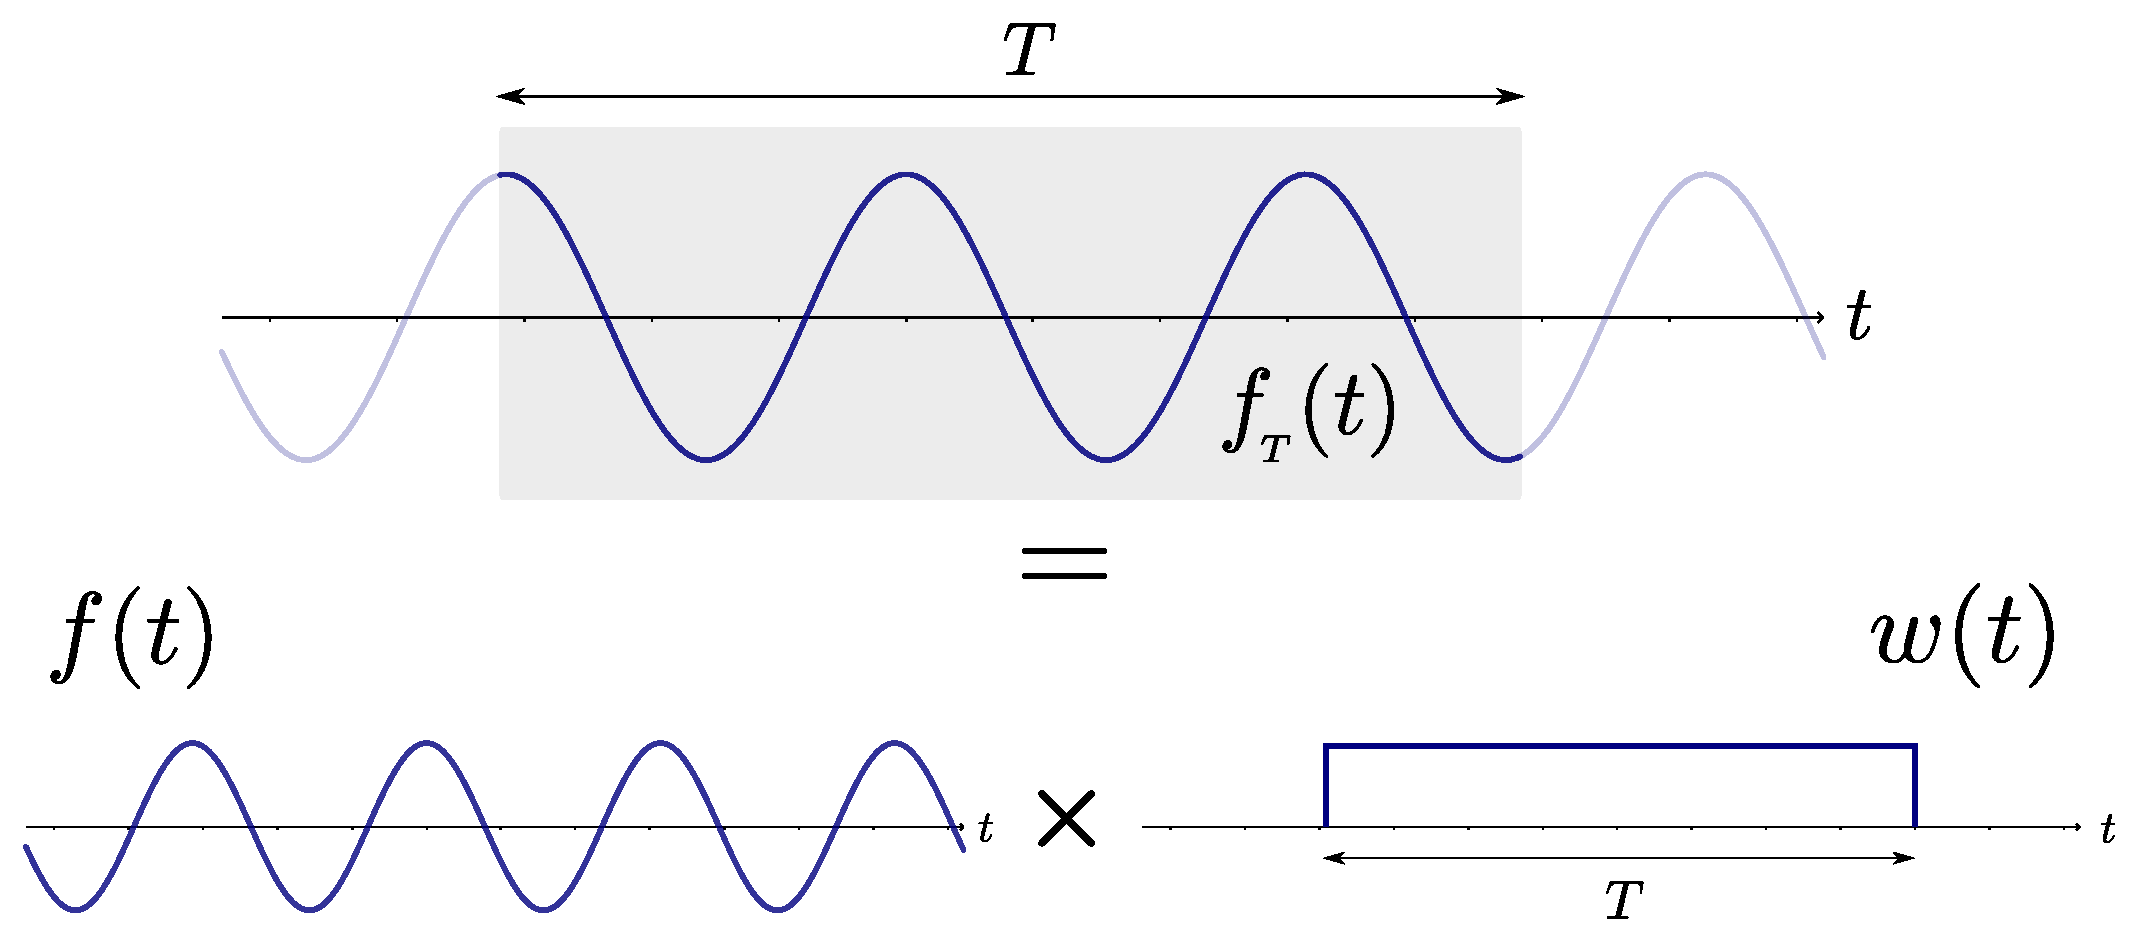
\includegraphics[width=\linewidth]{sampling-sine.pdf}
    \caption{Depiction of sampling as a multiplication with a finite window function}
    \label{fig:sampling-sine}
\end{figure}

Consider now the impact of windowing as viewed in the frequency domain. The original carrier wave, \(f(t)\), which theoretically spans over all time, is perfectly impulsive. However, multiplication with the windowing function in time is equivalent to convolution with the window's spectrum in frequency. The exact details of this spectrum depend on the windowing function used, but for a simple rectangular function,
\begin{equation}
    w(t) = \textrm{rect}\bigg(\frac{t}{T}\bigg) \xLeftrightarrow{\quad\mathcal{F}\quad} W(\omega) = T \cdot \textrm{Sa}\bigg(\frac{\omega T}{2}\bigg)
\end{equation}
where \(\textrm{Sa}(x)=\frac{\sin{x}}{x}\).

\begin{figure}[htbp]
    \centering
    \def\svgwidth{\linewidth}
    {\setstretch{0.7} % Line spacing
        \input{../Images/sampling-sine-freq.pdf_tex}}
    \caption{Effect of windowing on spectrum}
    \label{fig:sampling-sine-freq}
\end{figure}

Instead, each carrier has an associated spectrum, and this spectrum influences the ability for one to demodulate the other carriers.

How, then, does that influence the ability to perform \gls{fdm}?

Suppose one has three carriers, each with a \(\textrm{Sa}(\omega) = \frac{\sin \omega}{\omega}\) spectrum. If the centre frequencies of these carriers are sufficiently distant from the others, there will be negligible interference from one spectrum's sidelobes to another spectrum's mainlobe. This is seen in Figure~\ref{fig:three-sincs-good-distance}.


\begin{figure}
    \centering
    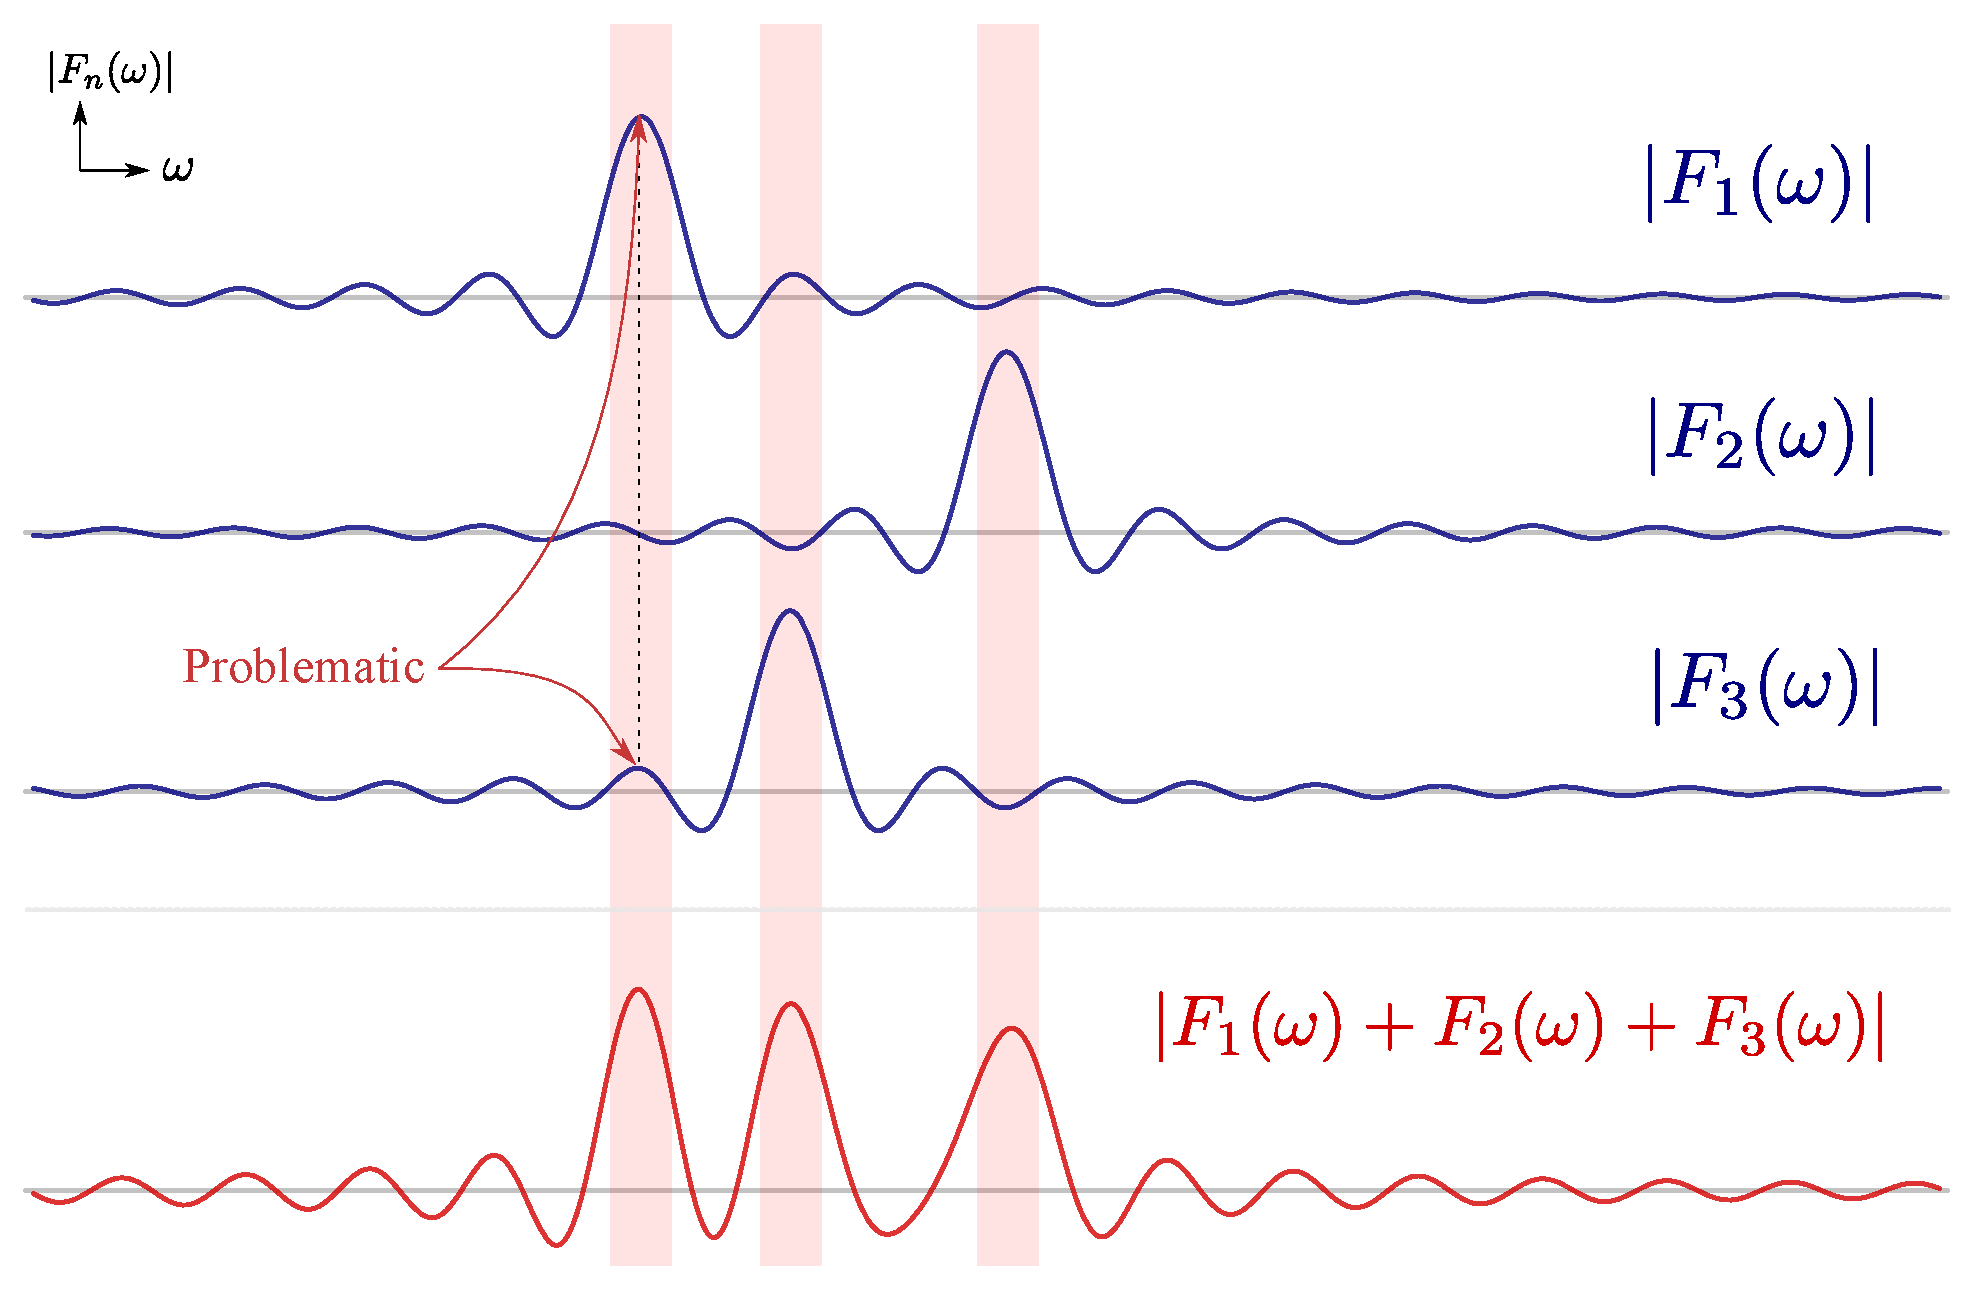
\includegraphics[width=\linewidth]{three-sincs-bad-distance.pdf}
    \caption{Three spectra spaced insufficiently far away from each other}
    \label{fig:three-sincs-bad-distance}
\end{figure}

\begin{figure}[htbp]
    \centering
    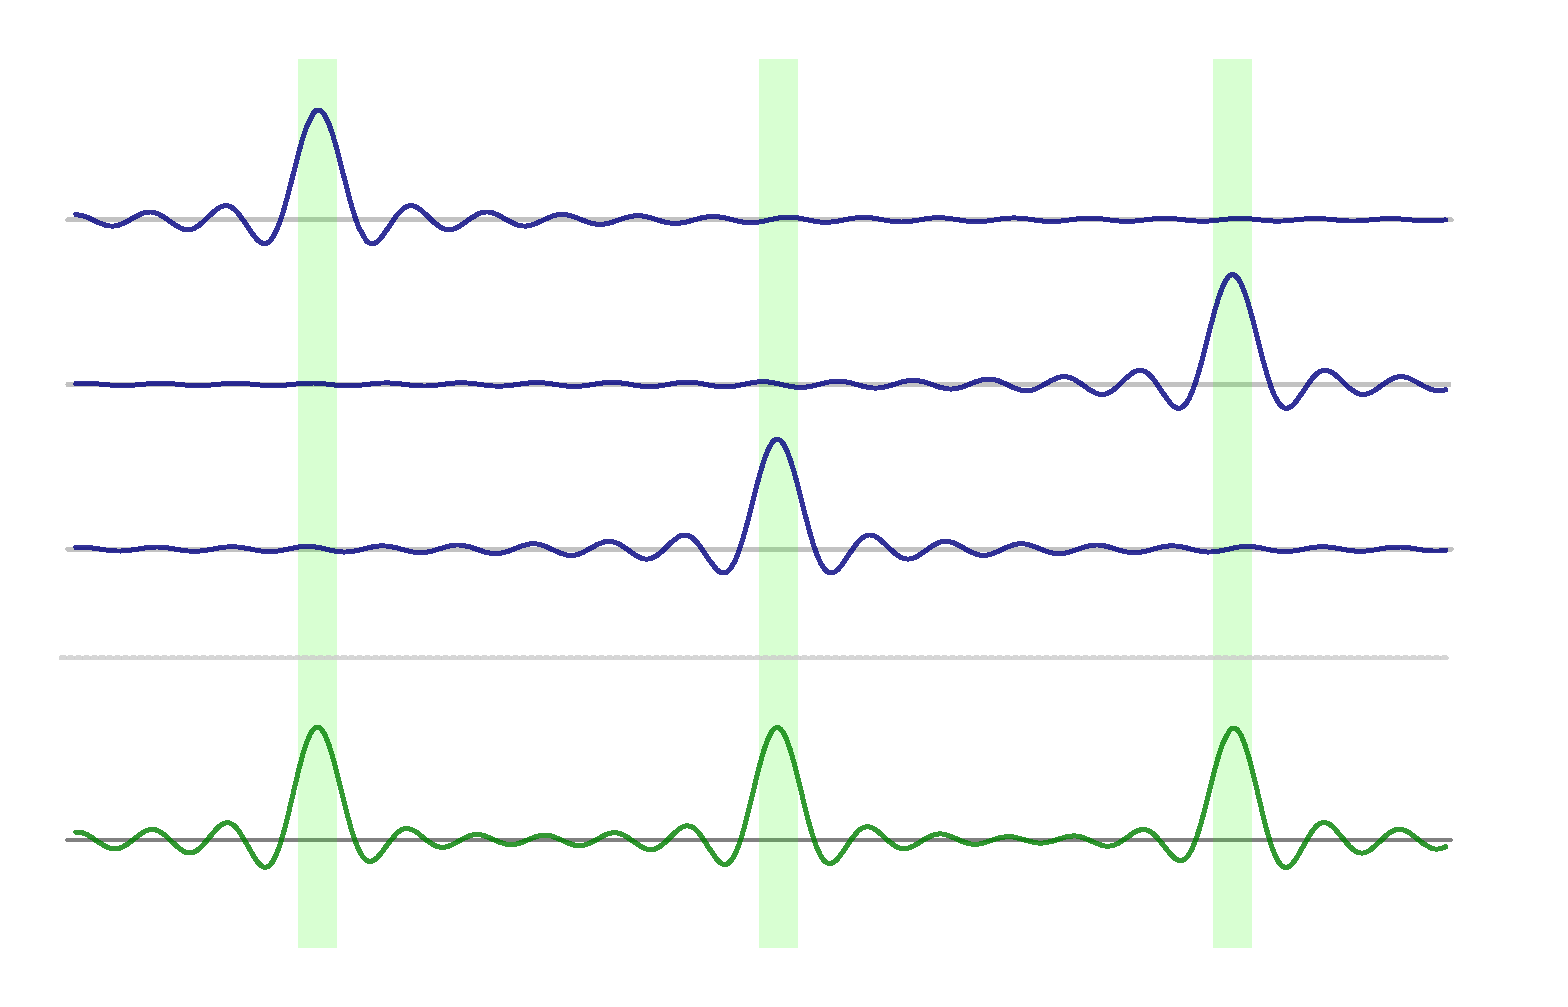
\includegraphics[width=\linewidth]{three-sincs-good-distance.pdf}
    \caption{Three spectra spaced sufficiently far away from each other}
    \label{fig:three-sincs-good-distance}
\end{figure}



\subsection{Using Orthogonal Carriers}
As shown, a straightforward \gls{fdm} approach requires the carriers to be sufficiently spaced from each other, to avoid cross-talk. There is an important exception to this requirement, provided one chooses the carrier frequencies very carefully: specifically, by spacing the carriers precisely with \(\Delta \omega = \frac{2\pi}{T}\). This is shown graphically in Figure~\ref{fig:ofdm-three-sincs}.

\begin{figure}[htbp]
    \centering
    \def\svgwidth{1\linewidth}
    {\setstretch{0.7} % Line spacing
        \input{../Images/ofdm-three-sincs.pdf_tex}}
    \caption{Three spectra arranged orthogonally}
    \label{fig:ofdm-three-sincs}
\end{figure}

Notice how the peak of each carrier wave is perfectly aligned with the zero crossings of the other carriers---resulting in zero cross-talk at those frequencies. Mathematically, choosing the carrier waves in this way results in the signals being \emph{orthogonal}. For detailed proofs of how this happens, see appendices%~\ref{sect:proofs_ofdm-time} and~\ref{sect:proofs_ofdm-freq}.

\subsection{Leveraging the Discrete Fourier Transform}
While the \gls{ofdm} system is conceptually clever, it was not adopted for some time due to practical constraints. Suppose one had \(K\) independent bitstreams to be modulated onto \(K\) carrier waves arranged orthogonally---an \gls{ofdm} transmission. In the time domain, this can be modelled as a sum of complex exponentials, and frequencies 
\begin{equation}    
    x(t) = \sum^K_{k} X_k e^{j k \omega_0 t}
\end{equation}
Consider a discrete representation of \(x(t)\), sampled at \(\frac{1}{T}\),
\begin{equation}
    x[n] = x(nT) = \sum^K_{k} X_k e^{j k \omega_0 nT}
\end{equation}


\begin{figure}
    \centering
    \def\svgwidth{\linewidth}
    {
        \setstretch{0.7} % Line spacing
        \scriptsize
        \input{../Images/ofdm-multipliers.pdf_tex}
    }
    \caption{Depicting of a multiplier approach to \gls{ofdm}}
    \label{fig:ofdm-multipliers}
\end{figure}


How could one perform this modulation process efficiently? Moreover, at the receiver end, how could one demodulate, and thus extract, the \(K\) bitstreams?

\subsection{Cyclic Prefixing and Guard Intervals}

\begin{figure}[htbp]
    \centering
    \def\svgwidth{1\linewidth}
    {\setstretch{0.7} % Line spacing
        \input{../Images/cyclic-prefix.pdf_tex}}
    \caption{}
    \label{fig:cyclic-prefix}
\end{figure}

Note: still same sampling period!


\subsection{Time \& Frequency Interleaving}
In a multipath situation, as discussed in section~\ref{subsect:multipath}, there is a problem of inter-symbol interference. These effects are mitigated in the \gls{dab} standard by utilizing the \gls{ofdm} scheme, together with cyclic prefixing. There is an additional problem, however. 

\begin{figure}[htbp]
    \centering
    \def\svgwidth{1\linewidth}
    {\setstretch{0.7} % Line spacing
        \input{../Images/ofdm-selective-fading.pdf_tex}}
    \caption{}
    \label{fig:ofdm-selective-fading}
\end{figure}


\subsection{Forward Error Correction}

\section{Differential Quadrature Phase Shift Keying \label{sect:dab-std_psk}}

The \gls{dab} standard utilizes a modulation technique called \acrlong{psk}, specifically a variant thereof called \(\frac{\pi}{4}-\)\gls{dqpsk}.

\subsection{Binary Phase Shift Keying}
Consider a sinusoidal carrier wave with a frequency of \(\omega_0\) and an amplitude of \(A\). Unlike in \gls{ask}---where the amplitude of the carrier wave is modulated, and in \gls{fsk}---where the frequency of the carrier wave is modulated, \gls{psk} keeps both the amplitude and frequency constant over time. Instead, it modulates the \emph{phase} of the carrier wave. Mathematically,
\begin{equation}
    f(t, n) = A \cdot \sin(\omega_0t + \phi[n])
\end{equation}
where \(\phi[n]\) is the corresponding phase for the symbol at the discrete-time step \(n\).

In the simplest case, one could take a bitstream of values---either 0 or 1---and correspondingly modulate the carrier with a phase of either~\(0\) or \(\pi\) radians. Such an approach is called \emph{binary} phase-shift keying, since only two values are used. Figure~\ref{fig:binary-psk} shows a simple example of this.

\begin{figure}[htbp]
    \centering
    \def\svgwidth{1\linewidth}
    {\setstretch{0.7} % Line spacing
        \input{../Images/binary-psk.pdf_tex}}
    \caption{Example of binary phase shift keying}
    \label{fig:binary-psk}
\end{figure}

\subsection{Differential Modulation}
In order to be demodulate a \gls{qpsk} signal properly, a receiver must be "fully coherent,"~\cite{Moosea}.

Otherwise, phase ambiguity problems.

% Notice in the previous example that the demodulator would need to have knowledge about the

\begin{figure}[htbp]
    \centering
    \def\svgwidth{1\linewidth}
    {\setstretch{0.7} % Line spacing
        \input{../Images/differential-binary-psk.pdf_tex}}
    \caption{Example of differential binary phase shift keying}
    \label{fig:differential-binary-psk}
\end{figure}

\subsection{Quadrature Phase Shift Keying}

\subsection{Adding $\pi/4$ Phase Offset}

\section{Transmission Frame}

\subsection{Overview}


\subsection{Null Symbol}


\subsection{Phase Reference Symbol}


\subsection{Data-carrying Symbols}



\section{Summary}


% ----------------------------------------------------
\ifstandalone
\bibliography{../Bibliography/References.bib}
\printnoidxglossary[type=\acronymtype]
\fi
\end{document}
% ----------------------------------------------------